\documentclass[main.tex]{subfiles}
%\date{9/4/22}
%\usepackage{tikz}
%\usetikzlibrary{positioning,calc}
%\usepackage{pgfplots}

\begin{document}
\subsubsection*{1. The Sun's Position at Noon}
In groups of 2-3, follow along the steps demonstrated by the instructor.
\begin{enumerate}[a.]
\item Set up Stellarium
	\begin{enumerate}[i.]
	\item Open the Location window and set the location to Amherst Center.
	\item Open the Sky and Viewing Options window.
		\begin{enumerate}[a)]
		\item Under the ``Sky" tab,
			\begin{enumerate}[1)]
			\item Set ``Stars Absolute Scale" to 0.0 (or the lowest it will go)
			\item Uncheck ``Show Atmosphere"
			\item Under ``Projection", select ``Cylinder"
			\end{enumerate}
		\item Under the ``Markings" tab,
			\begin{enumerate}[1)]
			\item Check ``Azimuthal Grid"
			\item Check ``Meridian"
			\end{enumerate}
		\end{enumerate}
	\item Zoom all the way out while staying centered on the South horizon point.
	\item Open Date/Time window and change the date to 21 September.
	\item Find the time (to within a few minutes) when the Sun is crossing the meridian (azimuth \SI{0}{\degree}00\si{\arcminute} or \SI{180}{\degree}00\si{\arcminute}, running from due north to due south). What time is it? What might cause it to \textbf{not} be 12:00 noon?
	\end{enumerate}

\item Plot the \textbf{altitude} of the Sun as it \textbf{crosses the meridian} on the 21st of each month throughout the year.
\end{enumerate}

\subsubsection{The Sun's Path during the Day}
Watch the Sun's path across the sky on 21 June and 21 December (the summer and winter solstices) over the whole day. On these dates, the Sun reaches its extreme north and south positions respectively. You can advance time faster or slower (or reverse it) using the and buttons in the bottom menu bar, or by \textbf{pressing the L and J keys}. Discuss what you see in your groups and answer the following questions:
\begin{enumerate}[a.]
\item The Sun does not always set due west! What azimuth range do you see it setting over?\\

\rule{15cm}{.2mm}

\item The Sun doesn't approach the horizon going straight down! Sketch what you see in Stellarium. Is the angle the same at both solstices?\\

\rule{15cm}{.2mm}

\item What is the Sun's azimuth at sunset on the equinoxes (22 September and 20 March)? (If there is ``landscape" in the way, look for when the Sun's altitude is near zero.)\\

\rule{15cm}{.2mm}

\item Suppose there are mountains rising to an altitude of \SI{10}{\degree} to the west. How would that affect the azimuth of sunset (when the Sun passes behind the landscape, including mountains) on the equinox?\\

\rule{15cm}{.2mm}

\end{enumerate}

\subsubsection{The Sun's Position at Different Latitudes}
Work in pairs and have one person do each part. Then, plot the Sun's noontime altitude throughout the year for both parts in the grid. (Make sure to record the values for the quiz.)

Note: when seen from the southern hemisphere, the Sun crosses the meridian in the \textbf{northern} sky!
\begin{center}
\begin{tabular}{|p{6cm}|p{2cm}|p{4cm}|p{3cm}|}\hline
City & Latitude & Sun max. altitude & Month \\\hline
Pick a city between S \SIrange{24}{60}{\degree}:&&&\\
&&&\\
&&&\\\hline
Pick a city in the tropics (between N \SI{23}{\degree} and S \SI{23}{\degree}):&&&\\
&&&\\
&&&\\\hline
\end{tabular}
\end{center}

\begin{figure}[htb]
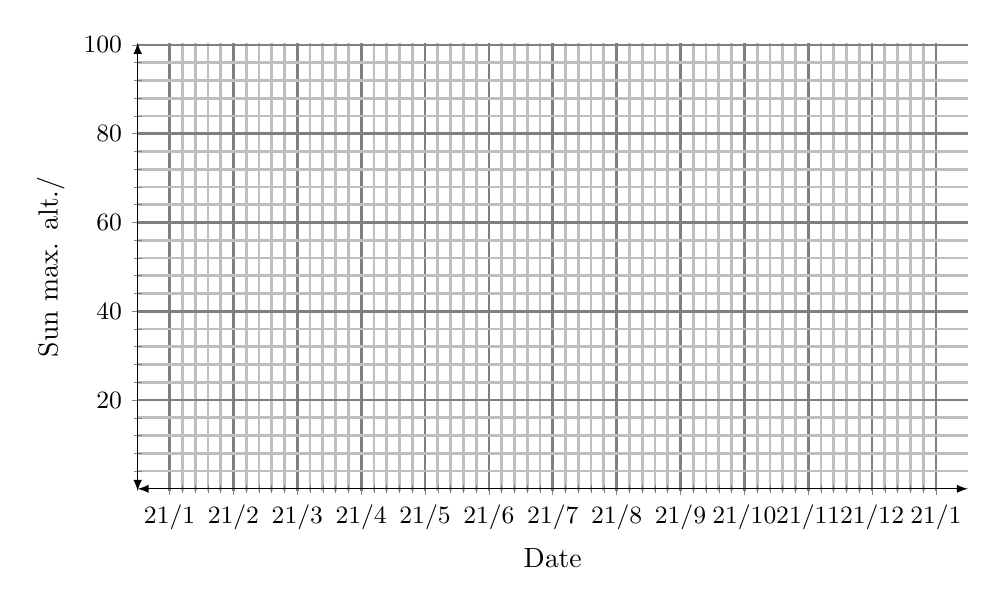
\begin{tikzpicture}
\begin{axis}[
	width=\textwidth,
    height=0.6\textwidth,
    xmin=1,xmax=13,
    ymin=0,ymax=100,
    grid=both,
    grid style={line width=1pt, draw=gray!50},
    major grid style={line width=1pt, draw=gray!100},
    axis lines=center,
    minor tick num=4,
    enlargelimits={abs=0.5},
    axis line style={latex-latex},
    xtick={1,2,3,4,5,6,7,8,9,10,11,12,13},
    xticklabels={21/1, 21/2, 21/3, 21/4, 21/5, 21/6, 21/7, 21/8, 21/9, 21/10, 21/11, 21/12, 21/1},
    ticklabel style={font=\small},
    xlabel near ticks,
    ylabel near ticks,
    xlabel={Date},
    ylabel={Sun max. alt./\si{\degree}}
]
\end{axis}
\end{tikzpicture}
\end{figure}

\subsubsection{The Sun's Path at Different Latitudes}
Now, let's look at how the Sun moves across the sky from different locations on Earth. Follow along with your instructor as below:

Open the Location window and type into the ``Latitude" entry ``N 66d 30m" (note where the spaces are). You should see the red arrow on the map jump to a location north of Amherst Center. (Leave the longitude unchanged from Amherst Center (W \SI{72}{\degree}) so the time zone stays the same.)
\begin{enumerate} [a.]
\item At the Arctic Circle (N \SI{66}{\degree} \SI{30}{\arcminute}) and northward, you can sometimes get 24 hours of daylight, and vice versa. Note how the Sun's path becomes more horizontal closer to the North Pole.

\item At the Equator (N \SI{0}{\degree}), notice how the Sun moves straight up and down as it approaches the horizon. Why would this make twilight shorter in the tropics?\\

\rule{15cm}{.2mm}


\item From locations at mid latitudes in the Southern Hemisphere, the Sun approaches the horizon at an opposite angle from what we see, and the Sun spends most of the day in the \textbf{northern} sky. Note: Does this mean that the Sun is travelling in the opposite \textbf{direction} (east or west)?\\

\rule{15cm}{.2mm}

\end{enumerate}

\subsubsection{Moodle Lab Quiz}
Go to the section for this lab on the Moodle page and complete the End-of-Lab Quiz. Note that some of the questions will depend on what city your team picked for part (3), so be sure to enter the correct latitude of that city.

%\textbf{Next Week:} Please bring the camera you plan to use for this semester's sunset project to lab next week so we can help you get started on completing the project successfully!
\end{document}